\hypertarget{oppgave2}{}
\section*{Oppgave 2}
\addcontentsline{toc}{section}{Oppgave 2}
I denne oppgaven genereres et sinusformet signal med ulik
samplingsfrekvens. Ved å endre steglengden kan vi se hvordan
antall samples per periode påvirker representasjonen av signalet.

% --------------------------------------------------
\subsection*{a)}
Først opprettes en tidsvektor fra 0 til 2 ms med en steglengde
på $5\,\mu s$. Samplingsfrekvensen finnes som den inverse av
steglengden:
\begin{verbatim}
dt = 5e-6; # s
fs = 1/dt; # samplingsfrekvens i Hz
t_start = 0; # s
t_end = 2e-3; # s

t = t_start:dt:t_end;
\end{verbatim}
Dette gir en samplingsfrekvens på:
\[
    f_s = \frac{1}{dt}
        = \frac{1}{5\mu s}
        = 200\,\text{kHz}
\]


% --------------------------------------------------
\subsection*{b)}

Signalet har en amplitude på 5 V og en frekvens på 2 kHz.
Vinkelfrekvensen beregnes fra $2\pi f$, og sinus-signalet
genereres deretter fra tidsvektoren:
\begin{verbatim}
A = 5; # V
f = 2e3; # Hz
w = 2*pi*f;

s = A*sin(w*t);
\end{verbatim}
Signalet kan uttrykkes som:
\[
s(t) = 5\sin(2\pi\cdot2000t).
\]
\begin{figure}[H]
    \centering
    \includegraphics[width=0.9\textwidth]
    {skalert_vs_ikks_skalert.png}
    \caption{Sinussignalet med tidsaksen vist i sekunder og millisekunder.}
\end{figure}

% --------------------------------------------------
\subsection*{c)--f)}

For å undersøke hvordan samplingen påvirker signalet brukes fire
forskjellige steglengder. For hver steglengde beregnes den
tilsvarende samplingsfrekvensen, tidsvektoren og det samplede
sinussignalet:
\begin{verbatim}
dts = [50e-6, 200e-6, 250e-6, 400e-6]; # steg lengder/sample perioder
for i = 1:length(dts);
    dt_i = dts(i);
    fs_i = 1/dt_i;
    t_i = t_start:dt_i:t_end;
    s_i = A*sin(w*t_i);
    spp_i = fs_i/f; # sample pr periode
end;
\end{verbatim}
Antall samples per periode kan finnes fra forholdet:
\[
\text{spp} = \frac{f_s}{f}
\]
Når steglengden øker, reduseres samplingsfrekvensen og dermed også antall samples som beskriver hver periode av signalet. Figuren under sammenligner de fire steglengdene i samme diagram.
\begin{figure}[H]
    \centering
    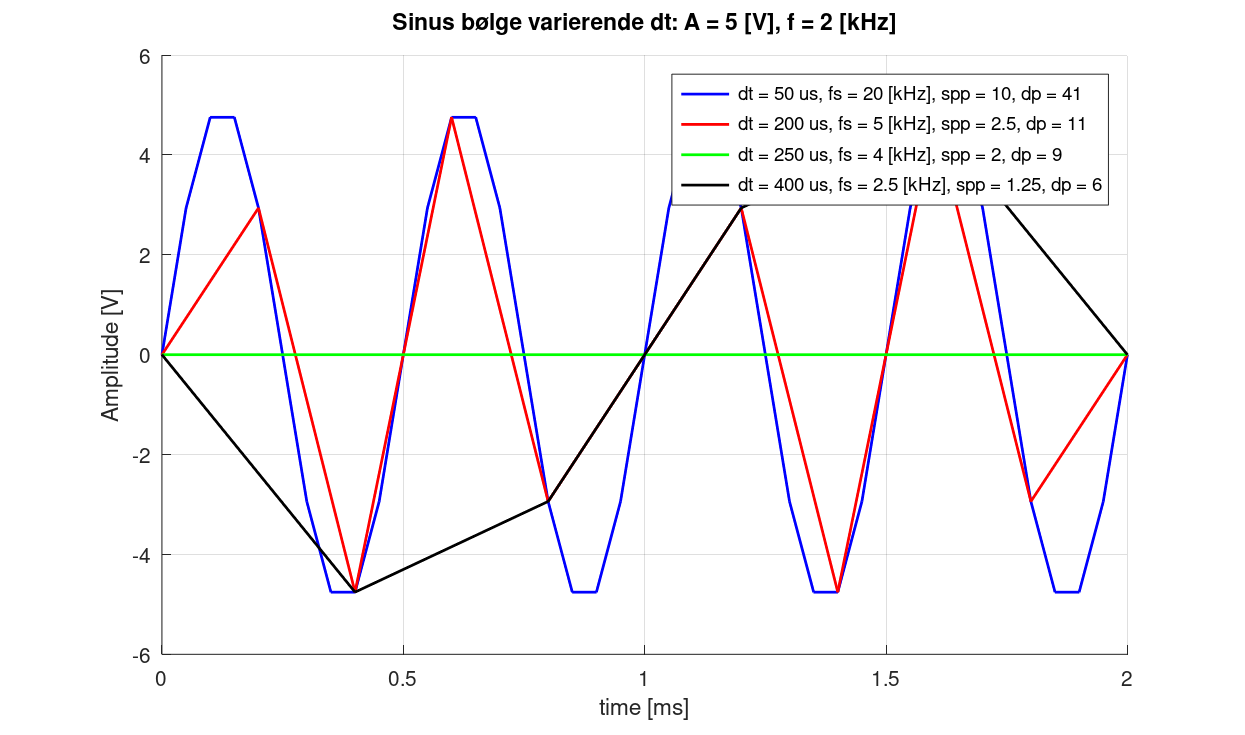
\includegraphics[width=0.9\textwidth]
    {Media/sammenlignei_dt_i_en_plot.png}
    \caption{Sammenligning av sinussignalet ved ulike steglengder.}
\end{figure}
\noindent De samme signalene vises også separat for å gjøre forskjellen mellom de ulike samplingsfrekvensene tydeligere.
\begin{figure}[H]
    \centering
    \includegraphics[width=1\textwidth]
    {fixedd_subplot_sammen_lignig_av_dt.png}
    \caption{De fire samplingsfrekvensene vist i separate diagrammer.}
\end{figure}
\noindent Ved $spp = 2$ er samplingsfrekvensen akkurat lik Nyquist-frekvensen. I dette tilfellet treffer samplingspunktene nullgjennomgangene til sinusbølgen, og signalet kan derfor ikke rekonstrueres fra de samplede verdiene. Dette viser hvorfor det i praksis er ønskelig med en samplingsfrekvens høyere enn $2f$.